\chapter{Задание 2. Комплексное}
\label{ch:chap3}

\definecolor{codegreen}{rgb}{0,0.6,0}
\definecolor{codegray}{rgb}{0.5,0.5,0.5}
\definecolor{codepurple}{rgb}{0.58,0,0.82}
\definecolor{backcolour}{rgb}{0.95,0.95,0.92}

\lstdefinestyle{mystyle}{
    backgroundcolor=\color{backcolour},   
    commentstyle=\color{codegreen},
    keywordstyle=\color{magenta},
    numberstyle=\tiny\color{codegray},
    stringstyle=\color{codepurple},
    basicstyle=\ttfamily\footnotesize,
    breakatwhitespace=false,         
    breaklines=true,                 
    captionpos=b,                    
    keepspaces=true,                 
    numbers=left,                    
    numbersep=5pt,                  
    showspaces=false,                
    showstringspaces=false,
    showtabs=false,                  
    tabsize=2
}

\lstset{style=mystyle}

\textit{NB.} - В этом задании мы используем унитарное преобразование Фурье к обычной частоте $\nu$, оно будет выглядеть следующим образом: 
\begin{align*}
    f(t) = \int_{-\infty}^{+\infty}\hat{f}(\nu)e^{2\pi i \nu t}dt \\
    \hat{f}(\nu) = \int_{-\infty}^{+\infty}f(t)e^{-2\pi i \nu t}dt
\end{align*}

Выберем треугольную функцию и зафиксируем для неё  $a$, $b$. После рассмотрим её сдвиг $g(t) = f(t + c)$.

\section{Фурье-образ}

Воспользуемся хитростью, а именно свойством Фурье-оператора:
$$
\mathbb{F}\{f(t+\tau)\} = e^{i \omega\tau}\mathbb{F}\{f(t)\}
$$, где $\tau$- наш сдвиг. 

В нашем случае его можно трактовать как \textit{поворот} образа в комплексной плоскости... Поэтому образ и приобретёт комплексную гармонику.

Образ Фурье будет выглядеть так:
$$
\hat{g}(\nu) = \frac{ab}{\sqrt{2\pi}}sinc^2(\frac{b\omega}{2})e^{i\omega\tau}
$$


\section{Графики функции, компонент f(t), а также её модуля}

\begin{figure}[ht]
    \centering
    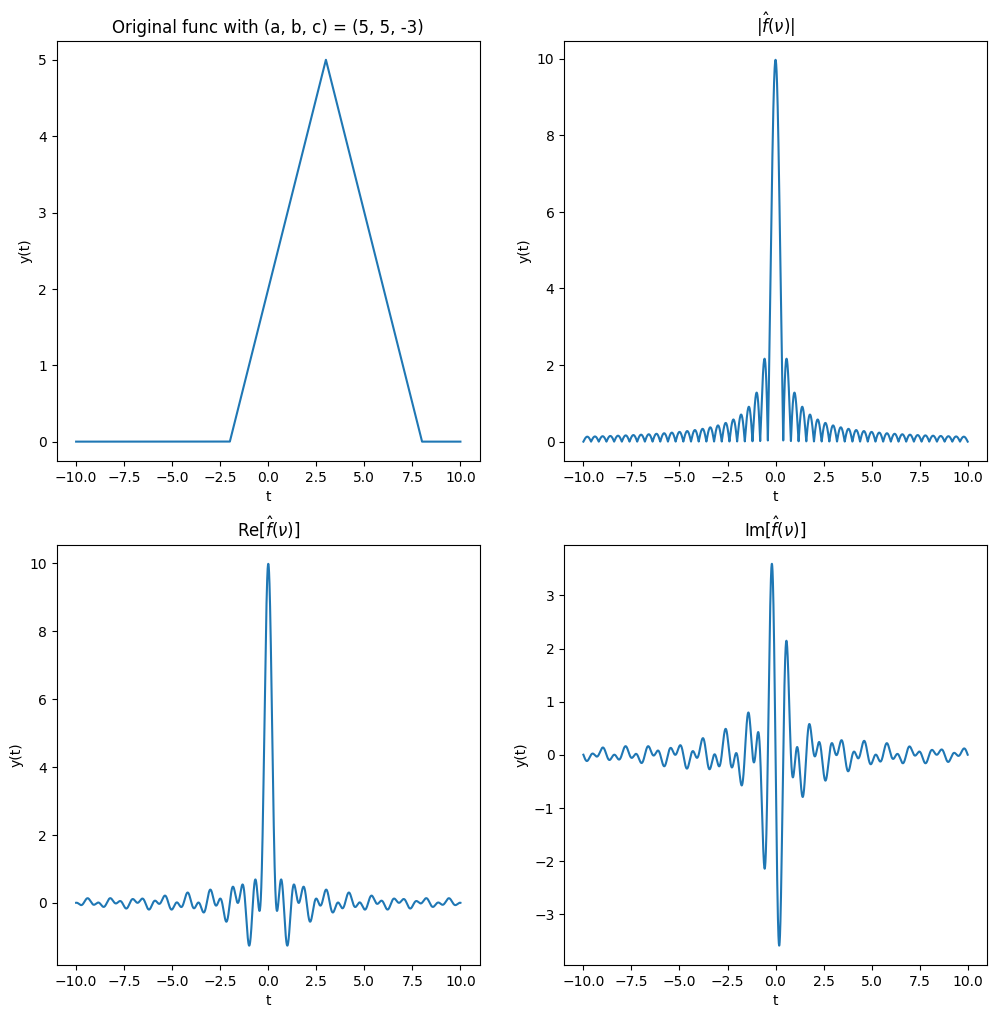
\includegraphics[width=1\textwidth]{f6_1.png}
    \caption{Общий план для комплексной функции}
\end{figure}

\begin{figure}[ht]
    \centering
    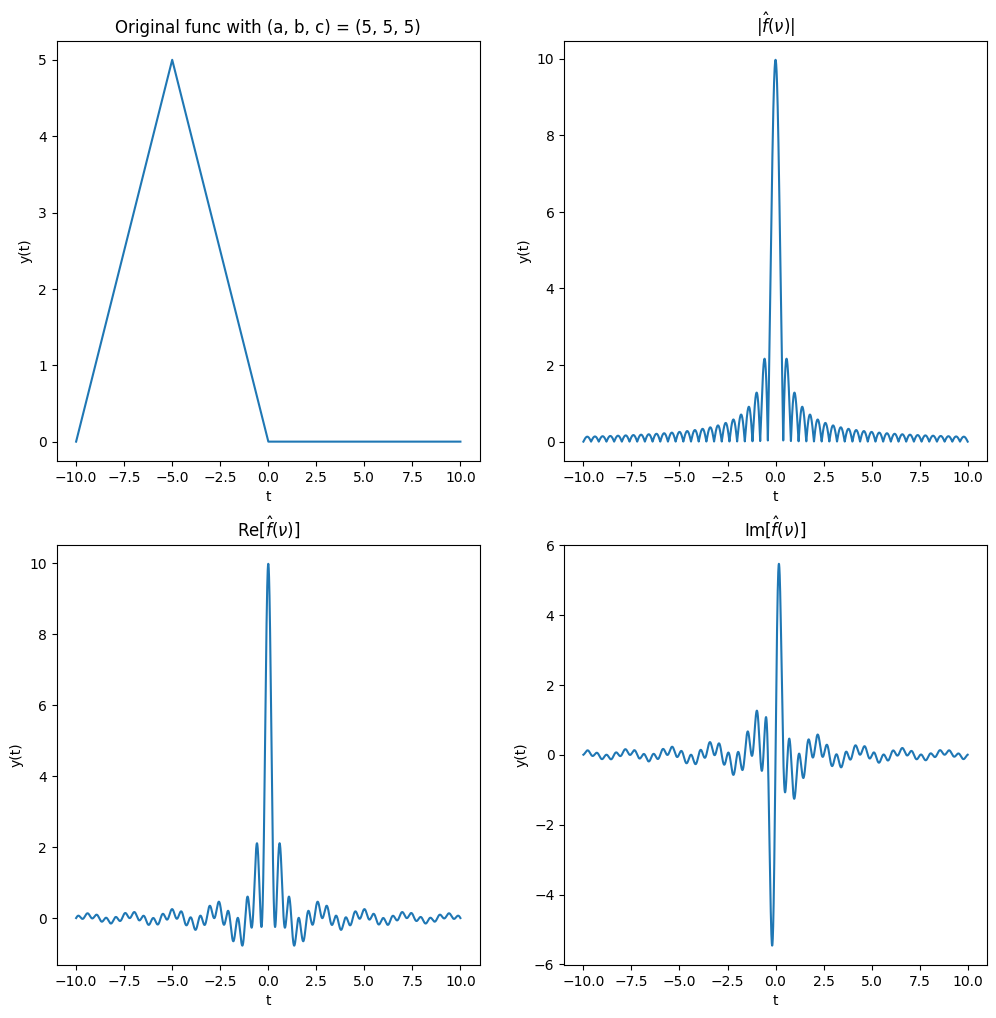
\includegraphics[width=1\textwidth]{f6_2.png}
    \caption{Общий план для комплексной функции}
\end{figure}

\begin{figure}[ht]
    \centering
    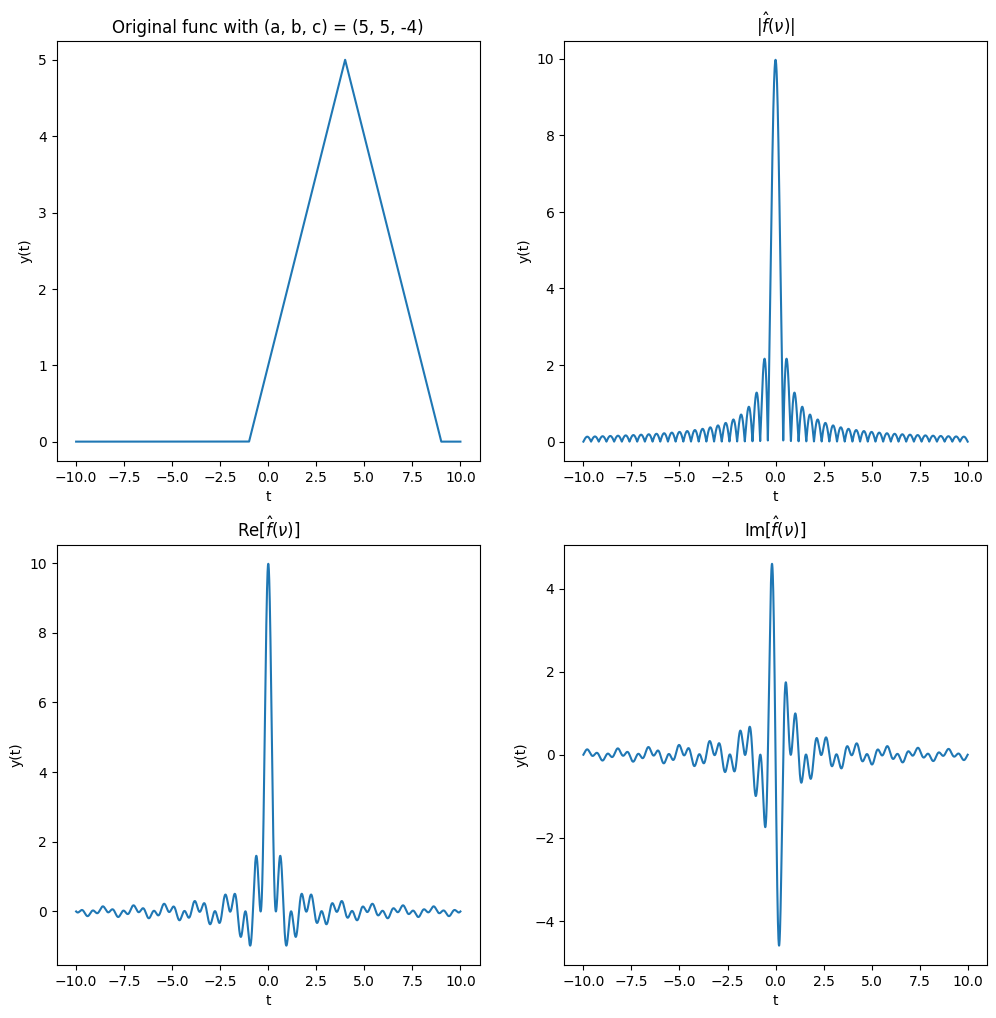
\includegraphics[width=1\textwidth]{f6_3.png}
    \caption{Общий план для комплексной функции}
\end{figure}

\begin{figure}[ht]
    \centering
    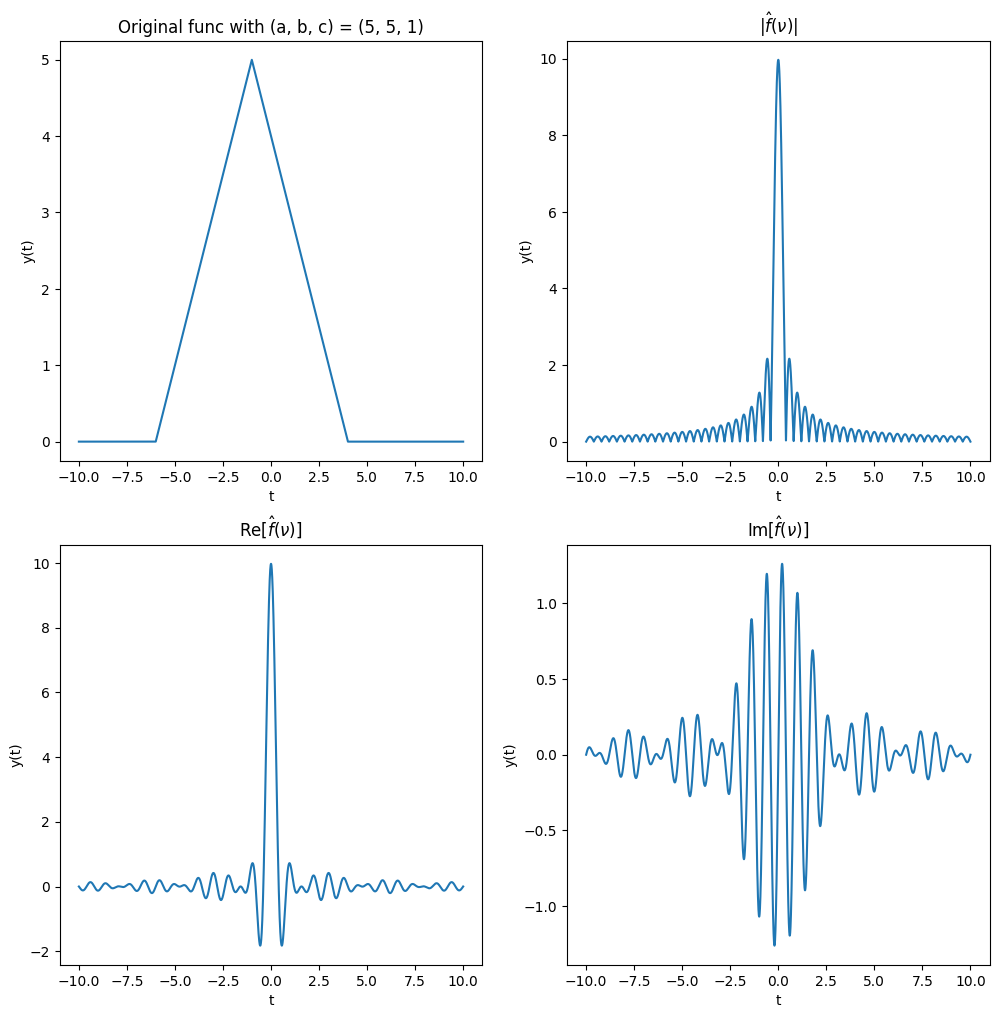
\includegraphics[width=1\textwidth]{f6_5.png}
    \caption{Общий план для комплексной функции}
\end{figure}

\begin{figure}[ht]
    \centering
    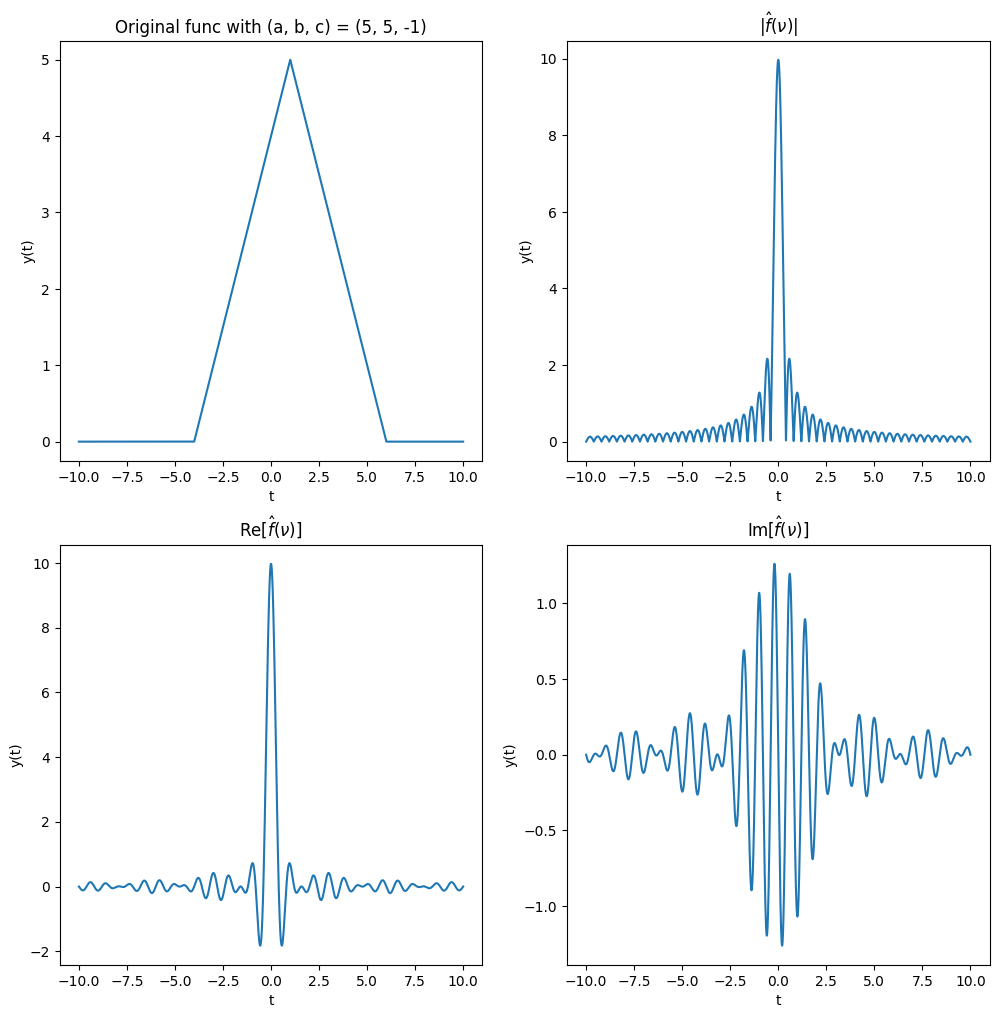
\includegraphics[width=1\textwidth]{f6_6.png}
    \caption{Общий план для комплексной функции}
\end{figure}

\begin{figure}[ht]
    \centering
    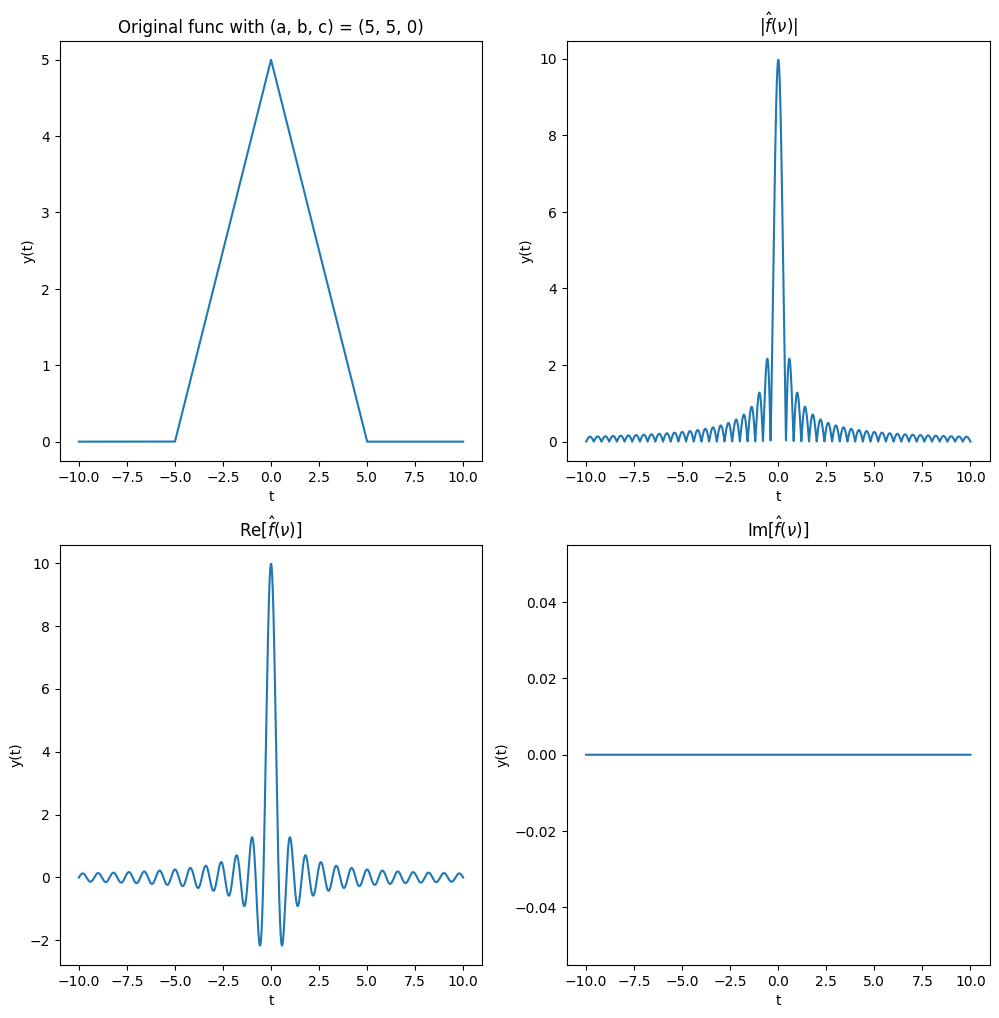
\includegraphics[width=1\textwidth]{f6_4.png}
    \caption{Общий план для комплексной функции}
\end{figure}

\section{Анализ степени сдвига на функцию и Фурье-образ}

Первое за что цепляется глаз - график модуля во всех случаях при фиксированных $a,b$ остаётся одним и тем же, после - сдвиг вправо или влево влияет только на направление гармоник, по модулю они остаются такими же (вещественна и комплексная). 
Поэтому при увеличении $c$ в какую-либо сторону заметна общая тенденция - обе гармоники сжимаются, но при этом график модуля по прежнему остаётся тем же.

Как бонус, проверили на последнем графике, что при $c=0$ мы возвращаемся в задание номер один, потому что комплексная компонента зануляется.

\section{Равенство Парсеваля}

Получил \texttt{delta: 0.00468}, довольно неплохое приближение, очевидно, что оно останется таким же и для других коэффициентов сдвига, было проверено для $c=\{1,5,-3\}$

\endinput